\documentclass[a4paper, 12pt]{article}
\usepackage[utf8]{inputenc}

%images
\usepackage{graphicx}       %for inserting images
\graphicspath{{../outputs/}}
\graphicspath{./}    %image file directory
\usepackage{wrapfig}
\usepackage{amsmath}
\usepackage{amssymb}
\usepackage{mwe}
\usepackage{listings} %for python code display
\usepackage{hyperref}	%hyperlink insertion
\usepackage{caption}	%caption

\captionsetup{
	font=small,
	labelfont=bf,
	tableposition=top
}
\usepackage{subcaption}	%for subfigures
\usepackage{geometry}
\geometry{margin = 0.7in}

%headers and footers
% All page numbers positioned at the bottom of the page
\usepackage{fancyhdr}
\fancyhf{} % clear all header and footers
\fancyfoot[C]{\thepage}
\fancyhead[R]{A. Thieshanthan, 180641N}   %header
\fancyhead[L]{\textbf{EN2550}}
\fancyhead[C]{Assignment A04}
\renewcommand{\headrulewidth}{1.5pt} % remove the header rule
\pagestyle{fancy}

%for inserting columns
\usepackage{multicol}       
\setlength{\columnsep}{1cm}

\usepackage{fancyvrb}
\usepackage{color}

\usepackage[backend = biber, style = ieee]{biblatex}
\addbibresource{reference.bib}

%opening
\title{Assignment A04: Neural Networks}
\author{A. Thieshanthan, 180641N}

\begin{document}
	
	\maketitle
	
	\begin{abstract}
		
	\end{abstract}

	\section{Linear Classifier}
		For this linear classifier, the scoring function $f(x)=Wx+b$ is used with the loss function Mean sum of squared errors(MSE). Some preparation and pre processing has been done to ease the coding and improve results. In some parts of the code numpy equivalent tensorflow functions are used to run the training on GPU.
		\subsection{Preparing dataset and Initializing parameters}
			The dataset images are normalized to produce a better effect on training. Normalizing is done by dividing by 255(largest entry in an image) and subtracting the mean of entire training set. Image labels are converted to one hot encoding vectors, which eases the loss computation. As there are 50000 training samples(m) with each image of size $32 \times 32\times 3$ the training dataset is reshaped into (3072, 50000) vector. This prepared dataset is used for Questions 1,2 and 3 of this assignment.
			\par 
			Weights $W$ and $b$ are initialized to random values as per standard normal distribution and zeros respectively. A dictionary $linear_model_history$ is initialized to store the history of training.
		\subsection{Model}
			As this is a simple model adding extra features such as learning rate decay, shuffling training data and adding regularization are relatively easy processes. 
			\begin{align}
					\hat{y} & = Wx + b \\
					L &= \frac{1}{m}\sum{(\hat{Y}-Y)^2} - \frac{1}{m}\sum W^2
			\end{align}
			which results in following gradients,
			\begin{align*}
				\frac{dL}{dw} &= \frac{2}{m}(\hat{Y} - Y)X^T - \frac{2}{m}W\\
				\frac{dL}{db} &= \frac{2}{m}(\hat{Y} - Y)
			\end{align*}
		Using this gradients, gradient descent algorithm has been implemented.
		\subsection{Training the classifier}
			Training has been done for 300 epochs with regularization and learning rate decay. Learning rate is reduced every 100 epochs and shuffling the training is also carried out. The hyperparameters and results are listed below in table \ref{param1}.
			\begin{table}
				\centering
				\begin{tabular}{|c|c|}
					\hline
					Hyperparameters & Value \\
					\hline
					Initial Learning rate & 0.0015 \\
					decay	& 0.001 \\
					regularization factor & 0.01 \\
					\hline
				\end{tabular}
				\label{param1}
				\caption{Hyperparameters for Linear Classifier}
			\end{table}
		\subsection{Results}
			\begin{table}
				\centering
				\begin{tabular}{|c|c|c|c|c|}
					\hline
					epoch & Training Loss & Training accuracy & Testing loss & Testing accuracy\\
					\hline
					1 & 1.0081 & 7.194 & 0.9988 & 11.55 \\
					300 & 0.8415 & 35.354 & 0.8410 & 35.25\\
					\hline
				\end{tabular}
				\caption{Training and testing loss and accuracy}
			\end{table}
			The trained weights are displayed as 10 images in figure \ref{fig:weights} and graphs of losses and accuracy are presented in figure \ref{label}
			\begin{figure}[h]
				\centering
				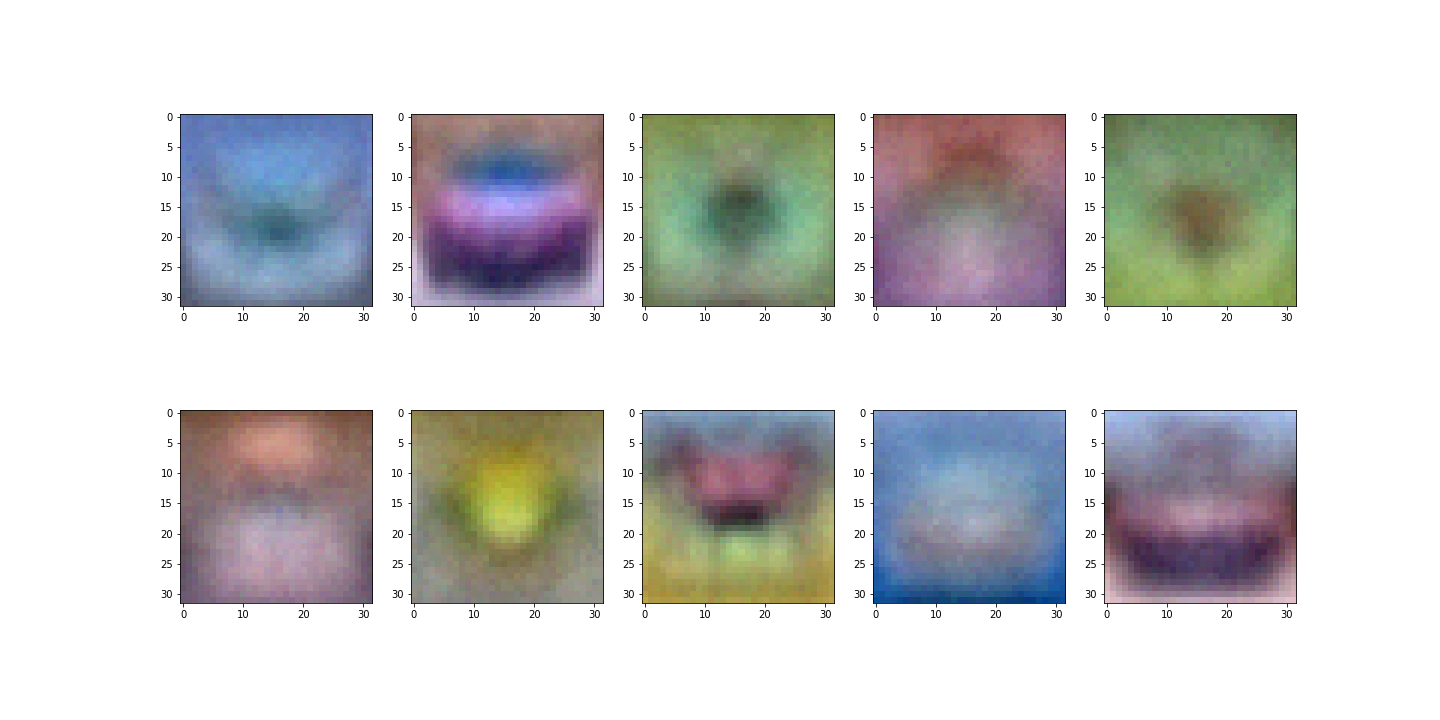
\includegraphics[scale = 0.4]{../images/weights}
				\caption{Trained weights of linear classifier}
				\label{fig:weights}
			\end{figure}
	
	
	\section{Two Layer Neural Network}
		A two layer neural network with sigmoid function as the activation function for the hidden layer has been implemented. There is no activation at the output layer and loss is MSE. 
		\subsection{Model}
			As the hidden layer has 200 units, the weights have been initialized with the shapes of [(200, 3072), (200,1)] and [(10,200), (10,1)] for each layer 1 and 2 respectively.
			\begin{align*}
				z_1 & = w_1X + b_1\\
				A_1 &= sigmoid(z1) \\
				\hat{Y} & = w_2A_1 + b_2 \\
				L &= \frac{1}{m}\sum{(\hat{Y}-Y)^2}  
			\end{align*}
		the derivatives related to each weight can be represented as follows using chain rule,
			\begin{align*}
				\frac{dL}{d\hat{Y}} &= \frac{2}{m}(\hat{Y} - Y) \\
				\frac{dL}{db_2} &= \frac{dL}{d\hat{Y}}\\
				\frac{dL}{dA_1} &= w_2^T\frac{dL}{d\hat{Y}}\\
				\frac{dL}{dz_1} &= \frac{dL}{dA_1} \times (A_1 * (1-A_1))\\
				\frac{dL}{dw_1} &= \frac{dL}{dz_1}X^T\\
				\frac{dL}{db_1} &= \frac{dL}{dz_1}\\
			\end{align*}
		Gradient descent algorithm has been implemented with these gradients.
		\subsection{Results}
		
		\begin{table}
			\centering
			\begin{tabular}{|c|c|c|c|c|}
				\hline
				epoch & Training Loss & Training accuracy & Testing loss & Testing accuracy\\
				\hline
				1 & 1.038 & 10.00 & 0.9389& 11 \\
				300 & 0.8566 & 27.36 & 0.8557 & 27.89\\
				\hline
			\end{tabular}
			\label{nn2}
			\caption{Training and testing loss and accuracy for 2 layer network}
		\end{table}
	
	\section{Implementing Stochastic Gradient Descent}
		The disadvantage of gradient descent algorithm is it waits until all the training data is used for one gradient calculation and then makes a progress. Stochastic Gradient Descent(SGD) update gradients for every sample processed. Which makes use of all the computations carried out and makes process towards reducing loss from step 1. But this introduces *** in training. Mini batches are used to solve this and helps to arrive at a converging point much faster than regular gradient descent. This can be observed by comparing losses and accuracies provided in table \ref{nn2} and table \ref{sgd}. 
		\par 
		It can be observed that SGD with minibatch outperforms regular gradient descent by a huge margin with given number of epochs. But using SGD somewhat increases the runtime of training but provides better results. SGD is useful when there is high number of training samples are available. It can also used when size of one training sample is very high and loading all the data at once is not possible.
		\begin{table}
			\centering
			\begin{tabular}{|c|c|c|c|c|}
				\hline
				epoch & Training Loss & Training accuracy & Testing loss & Testing accuracy\\
				\hline
				1 & 0.8902 & 13.2265 & 0.8390 & 12.16 \\
				300 & 0.7625 & 43.8878 & 0.7791 & 40.78\\
				\hline
				
			\end{tabular}
			
			\caption{Training and testing loss and accuracy for 2 layer network with SGD optimizer}
			\label{sgd}
		\end{table}
	
	\section{Convolutional Neural Network with Keras}
		A Convolutional Neural network(CNN) has been implemented with the given architecture. ReLu is used as activation for the convolutional layers and penultimate fully connected layer. Softmax function is used as the activation function of the last layer. SGD has been implemented with momentum of 0.01. 
		\par 
		As the convolutional layers extract features from the image, CNN outperform every network implemented from question 1 to 3. The results are provided in table \ref{tab:cnn}. The implemented CNN passes the training loss and accuracy of 2 layer network with a small number of epochs. But it overfits the training data hence the testing loss is increasing after several number of epochs.
	
\end{document}